\section{Introduction}

The main components used in this assignement is the \textit{EFM32GG Giant Gecko microcontroller} combined with
the \textit{ARM Cortex-M3 processor}, connected to a curcuit board containg eight LEDs and buttons. Both the 
micocontroller and the processor is designed to be highly energy efficient, and thus support five different energy modes.
Energy mode 0 provides full functionality, while energy mode 4 provides little functionality but uses a lot less power. 

\linebreak[4]
The assignment is as follows:

\begin{itemize}
    \item   Write an assembly program which enables a user to control the LEDs in some way by
            by pressing the buttons.
    \item   Write an interrupt rotuine (an interrupt handler) for reading the buttons.
    \item   Use a Makefile to compile and upload the program to the microcontroller.
    \item   Use the energy monitor to see the power requirements of your program. Analyze and
            discuss (or implement) improvements. 
    \end{itemize}


A processor is a machine that executes
a sequence of different instructions. The instructions are
single, independent calculations that makes little sense alone.
The order, or combination of the instructions, is what gives meaning to
the independent instructions and becomes a computer program.
Because the CPU only executes simple instructions, 
it has to execute a lot of them in order to be efficient. Thus,
the CPU is optimized to achieve a high throughput, 
i.e. to execute as many instructions as possible in the amount of time
that the processor is executing.

One of the most important optimization techniques on the modern CPU
is pipelining. The goal of adding a pipeline to
the CPU, is to have as little \textit{idle time} in the CPU's internal
components as possible. This is done by letting the CPU work on multiple
instructions at the same time, where \textit{each} instruction is being
worked on by a single \textit{part} of the pipeline, thereby achieving a higher
\textit{Instruction Level Parallelism}(ILP).

Most of the instructions in MIPS is built up of different stages,
A pipeline is achieved by adding specific \textit{pipeline registers} between
each of the different stages, where each of the registers contain all control
information that is needed by the instruction executing on the respective stage.
The different pipeline registers is named according to the different pipeline stages,
and is shown in Figure \ref{pipeline-registers}.

\begin{figure}[ht]
    \centering
      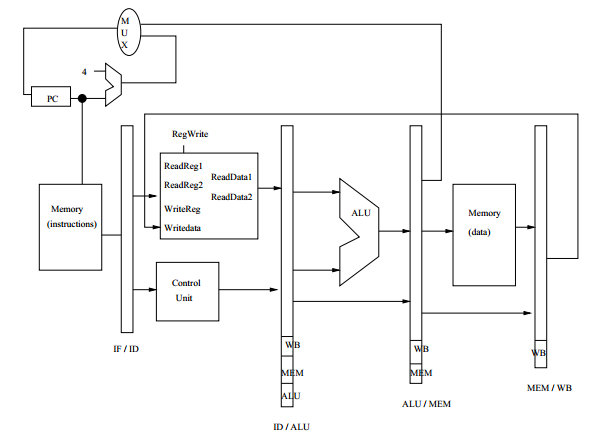
\includegraphics[width=9cm]{figures/pipeline-registers}
    \caption{A pipelined MIPS processor, with the respective registers between
        the different pipeline stages}
    \label{pipeline-registers}
\end{figure}

\begin{description}
    \item[Instruction Fetch/Instruction Decode] \hfill \\
        The IF/ID register contains the fetched instruction from instruction memory.
    \item[Instruction Decode/ALU] \hfill \\
        The ID/ALU contains the fetched instruction, plus controls that 
        are needed to execute the instruction. These control
        signals are available by the end of the ID stage and can be written into the pipeline register there - namely the register ID/ALU.
    \item[ALU/Memory] \hfill \\
        ALU/MEM register contains the controls that are needed to execute
        the remaining stages of the instruction (MEM, WB), as well as values 
        that were computed in the ALU stage.
    \item[Memory/Write Back] \hfill \\
        MEM/WB contains controls needed to execute the WB stage, as well as any data
        values that need to be written back.
\end{description}